\documentclass{beamer}

\usetheme[
  % Activates footline information (short title, short author).
  % fullfootline,
  % Sets a picture as the title background. If this option is not given, the primary color is used to create a solid background.
  % background=./graphics/forest.jpg,
  % The primary color to use for the theme. Defaults to Pantone 200 C
  % primaryColor = BA0C2F,
  % This is intended to be a lighter version of the primary color. Defaults to Pantone 431 C, 50%
  % primaryLightColor = DAE6EF,
	% secondaryColor = 5B6770,
]{miniuol}

% 150% Line Spacing
\linespread{1.213}

\title{The Title:}
\subtitle{There Is a Subtitle Too}
\date{\today}
\author{A. Author}
\institute{Institute}
\titlegraphic{
\includegraphics[width = 8em]{./graphics/uol-white.pdf}}
\begin{document}

\begin{frame}[plain, noframenumbering]
	\titlepage
\end{frame}

\begin{frame}{The \texttt{miniuol} beamer theme}
	\texttt{miniuol} is a minimal theme for the \LaTeX{} beamer document class that emphasizes simplicity, legibility and elegance.

	It has been forked from the \emph{Manc} theme (available at \url{https://github.com/ibab/beamertheme-manc}), with modifications to fit my taste.

	For instance, \emph{Manc} used the Fira typeface family throughout; that has been replaced with a combination of the San Francisco font stack and Iosevka Slab (as a monospaced font).
\end{frame}

\begin{frame}[fragile]
	\begin{columns}
		\begin{column}{0.5\textwidth}
			\begin{block}{Block}
				This is a simple block created using the \texttt{block} environment.
			\end{block}
			\begin{exampleblock}{Example block}
				This is an example block created using the \texttt{exampleblock} environment.
			\end{exampleblock}
		\end{column}
		\begin{column}{0.5\textwidth}
			\emph{Manc} replaces the default beamer blocks with boxes from the \href{https://www.ctan.org/pkg/tcolorbox}{\texttt{tcolorbox}} package.
			These can be configured in much more detail than a \texttt{beamercolorbox}
			\medskip

			Use boxes sparingly to highlight specific pieces of information (theorems, formulas, commands, …) that you want your audience to remember.\footnote[frame]{Add footnotes by using \texttt{\backslash footnote[frame]\{…\}}}
		\end{column}
	\end{columns}
\end{frame}

\begin{frame}
	\centering
	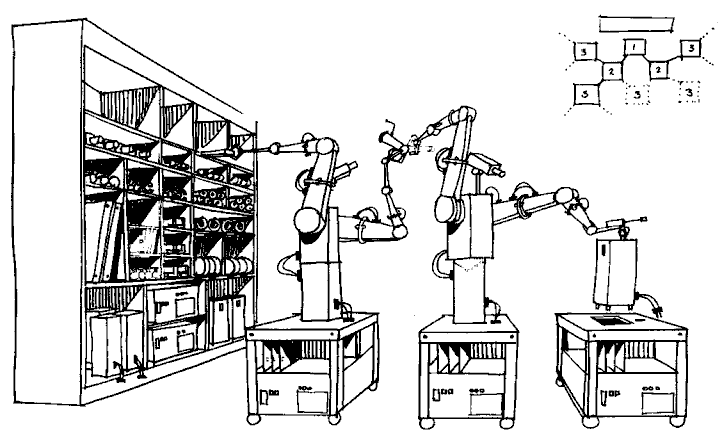
\includegraphics[width = \textwidth]{./graphics/self-replicating.png}
\end{frame}

\begin{frame}[fragile]
	\frametitle{A slide with code}
	Here is some R code:

\begin{verbatim}
# Plot using R-base
x <- runif(10)
y <- 2 * x + rnorm(10)
plot(x, y)
\end{verbatim}

\end{frame}

\begin{frame}
	\frametitle{A slide with some maths}
	Here a slide with some maths:

\[
y = a + \beta x + \varepsilon
\]

\end{frame}

\begin{frame}
	\frametitle{A slide with a quote}

	\begin{quote}
		Ball don't lie!
	\end{quote}

	...a wise man once said.

\end{frame}

\begin{frame}
	\frametitle{Frame with lists}

	\begin{enumerate}
		\item One;
		\item Two;
		\item Penny and a dime.
	\end{enumerate}

	\begin{itemize}
		\item Pizza;
		\item More pizza;
		\item Did I say I love pizza?
	\end{itemize}

\end{frame}

\begin{darkframe}[c, noframenumbering]
		\begin{tikzpicture}[overlay, remember picture]
		\node[anchor = center] at (current page.center) {
		\begin{beamercolorbox}[center]{title}
			\usebeamerfont{large text} Thank you.
		\end{beamercolorbox}};
		\end{tikzpicture}
\end{darkframe}

\end{document}
